\section{Clase 4}

\title[Circuitos Discretos]{Circuitos Discretos}
\subtitle{Clase 4: Emisor Común}
\institute[]{Instituto Tecnológico de Costa Rica\\Escuela de Ingeniería Electrónica\\Circuitos Discretos}
\date{\theSemester}
\titlegraphic{
\includegraphics[height=8mm]{logoTEC.png}}

\begin{frame}[t]
\titlepage
\end{frame}

\begin{frame}[t]
    \frametitle{Emisor Común}

    \begin{columns}
        \begin{column}{0.4\textwidth}
            \centering
            \begin{figure}[H]
                \begin{circuitikz}
                    \draw (0,0) node[npn](npn1){};
                    \draw (-1.5,0) to[short] (npn1.base);
                    \draw (-1.5,0) to[vsource,l=$v_{in}$] (-1.5,-2);
                    \draw (-1.5,-2) node[ground]{};
                    \draw (0,2) to[R,l=$R_C$] (npn1.collector);
                    \draw (0,0.5) to[short,-o] (1,0.5);
                    \draw (0,-1) node[ground]{};
                    \draw (0,-1) -- (npn1.emitter);
                    \draw (1,0.5) node[anchor=west]{$v_{out}$};
                    \draw (0,2.5) -- (0,2);
                    \draw (-0.5,2.5) -- (0.5,2.5);
                    \draw (0,2.5) node[anchor=south]{$V_{CC}$};
                \end{circuitikz}
            \end{figure}
        \end{column}
        \begin{column}{0.6\textwidth}
            Para la configuración de Emisor Común:

            \begin{itemize}
                \item La entrada se aplica en la base.
                \item La salida se toma del colector.
            \end{itemize}

            \vspace{5mm}

            Análisis cualitativo de $A_V$:

            \begin{enumerate}
                \item Si $v_{in}$ aumenta, $v_{BE}$ aumenta
                \item Si $v_{BE}$ aumenta, $i_c$ aumenta
                \item Si $i_c$ aumenta, $v_{RC}$ aumenta
                \item Si $v_{RC}$ aumenta, $v_{out}$ disminuye
            \end{enumerate}

            $\Rightarrow$ Un cambio positivo en $v_{in}$ reduce $v_{out}$

            $\Rightarrow$ La ganancia es negativa
        \end{column}
    \end{columns}
\end{frame}

\begin{frame}[t]
    \frametitle{Emisor Común: Ganancia del Núcleo}

    \begin{columns}
        \begin{column}{0.35\textwidth}
            1. LVK por la base
    
            \[ v_{in} = v_\pi \]

            2. LCK en el colector

            \[ g_m v_\pi + \dfrac{v_{out}}{R_C} = 0 \]

            3. Combinando 1 y 2:
    
            \[ g_m v_{in} + \dfrac{v_{out}}{R_C} = 0 \]

            \[ \dfrac{v_{out}}{R_C} = -g_m v_{in} \]

            \[ \boxed{A_V = \dfrac{v_{out}}{v_{in}} = -g_m R_C} \]
        \end{column}
        \begin{column}{0.65\textwidth}
            \centering
            \begin{figure}[H]
                \begin{circuitikz}
                    \draw (0,0) -- (1,0);
                    \draw (1,0) to[R,l=$r_\pi$,v=$v_\pi$] (1,-2);
                    \draw (1,-2) -- (3,-2);
                    \draw (3,0) to[cisource,l=$g_m v_\pi$] (3,-2);
                    \draw (3,0) -- (6,0);
                    \draw (2,-2) node[ground]{};
                    \draw (2,-2) node[anchor=south]{E};
                    \draw (1,0) node[anchor=south]{B};
                    \draw (5,0) node[anchor=south]{C};
                    \draw (0,0) node[anchor=east]{$v_{in}$};
                    \draw (6,0) node[anchor=west]{$v_{out}$};
                    \draw (5,0) to[R,l=$R_C$] (5,-2);
                    \draw (5,-2) node[ground]{};
                \end{circuitikz}
            \end{figure}

            \vspace{5mm}
            \begin{enumerate}
                \item La ganancia es negativa (la salida está invertida con respecto a la entrada).
                \item La ganancia es proporcional a $g_m$
            \end{enumerate}
            %
            \[ A_V \propto g_m \propto I_C \]
        \end{column}
    \end{columns}
\end{frame}

\begin{frame}[t]
    \frametitle{Emisor Común: Limitación de Ganancia}

    La tensión de salida es la tensión del colector.

    \begin{itemize}
        \item La tensión $V_C$ no puede ser más alta que $V_{CC}$ (tensión de fuente).
        \item La tensión $V_C$ no puede ser más baja que $V_{BE}$ (transistor en saturación).
    \end{itemize}

    \vspace{3mm}
    \begin{columns}
        \begin{column}{0.6\textwidth}
            Considere la ecuación de ganancia:
            
            \[ A_V = -g_m R_C \]

            La ganancia máxima de la configuración E.C. es:

            \[ A_V = -\left( \dfrac{I_C}{V_t} \right) \cdot \left( \dfrac{V_{RC}}{I_C} \right) \]

            \[ A_{Vmax} = -\left( \dfrac{I_C}{V_t} \right) \left( \dfrac{V_{CC}-V_{BE}}{I_C} \right) \]

            \[ \boxed{A_{Vmax} = - \dfrac{V_{CC}-V_{BE}}{V_t}} \]
        \end{column}
        \begin{column}{0.4\textwidth}
            \begin{figure}[H]
                \scalebox{0.8}{
                    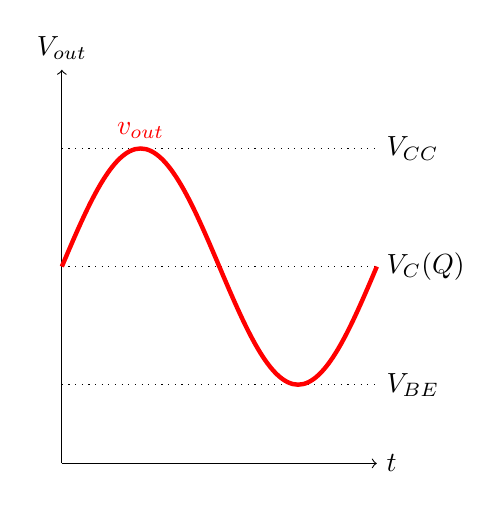
\begin{tikzpicture}
                        \draw[->] (0,0) -- (4,0); % x axis
                        \draw[->] (0,0) -- (0,5); % y axis
                        \draw (4,0) node[anchor=west]{$t$};
                        \draw (0,5) node[anchor=south]{$V_{out}$};
                        \draw[dotted] (0,1) -- (4,1); % V_{BE}
                        \draw (4,1) node[anchor=west]{$V_{BE}$};
                        \draw[dotted] (0,4) -- (4,4); % V_{CC}
                        \draw (4,4) node[anchor=west]{$V_{CC}$};
                        \draw[dotted] (0,2.5) -- (4,2.5); % V_C
                        \draw (4,2.5) node[anchor=west]{$V_C(Q)$};
                        \draw[ultra thick, red](0,2.5) sin (1,4) cos (2,2.5) sin (3,1) cos (4,2.5);
                        \draw[red] (1,4) node[anchor=south]{$v_{out}$};
                    \end{tikzpicture}
                }
                \caption{Amplitud máxima de $v_{out}$}
            \end{figure}
        \end{column}
    \end{columns}
\end{frame}

\begin{frame}[t]
    \frametitle{Emisor Común: Impedancias de Entrada y Salida}

    \begin{columns}
        \begin{column}{0.5\textwidth}
            \centering
            Impedancia de entrada

            (salida en circuito abierto)

            \begin{figure}[H]
                \scalebox{0.7}{
                \begin{circuitikz}
                    \draw (-1,0) -- (1,0);
                    \draw (-1,0) to[vsource,l=$v_x$,i=$i_x$] (-1,-2);
                    \draw (-1,-2) node[ground]{};
                    \draw (1,0) to[R,l=$r_\pi$,v=$v_\pi$] (1,-2);
                    \draw (1,-2) -- (3,-2);
                    \draw (3,0) to[cisource,l=$g_m v_\pi$] (3,-2);
                    \draw (3,0) -- (5,0);
                    \draw (2,-2) node[ground]{};
                    \draw (2,-2) node[anchor=south]{E};
                    \draw (1,0) node[anchor=south]{B};
                    \draw (3,0) node[anchor=south]{C};
                    \draw (5,0) to[R,l=$R_C$] (5,-2);
                    \draw (5,-2) node[ground]{};
                \end{circuitikz}
                }
            \end{figure}
            %
            \[ i_x = \dfrac{v_x}{r_\pi} \]
            %
            \[ \dfrac{v_x}{i_x} = r_\pi \]
            %
            \[ \boxed{R_{in} = r_\pi} \]
        \end{column}
        \begin{column}{0.5\textwidth}
            \centering
            Impedancia de salida

            (entrada en cortocircuito)
            
            \begin{figure}[H]
                \scalebox{0.7}{
                \begin{circuitikz}
                    \draw (0,0) -- (1,0);
                    \draw (1,0) to[R,l=$r_\pi$,v=$v_\pi$] (1,-2);
                    \draw (1,-2) -- (3,-2);
                    \draw (3,0) to[cisource,l=$g_m v_\pi$] (3,-2);
                    \draw (3,0) -- (7,0);
                    \draw (2,-2) node[ground]{};
                    \draw (2,-2) node[anchor=south]{E};
                    \draw (1,0) node[anchor=south]{B};
                    \draw (3,0) node[anchor=south]{C};
                    \draw (0,0) node[ground]{};
                    \draw (7,0) to[vsource,l=$v_x$,i=$i_x$] (7,-2);
                    \draw (7,-2) node[ground]{};
                    \draw (5,0) to[R,l=$R_C$] (5,-2);
                    \draw (5,-2) node[ground]{};
                \end{circuitikz}
                }
            \end{figure}
            %
            \[ v_\pi = 0 \]
            %
            \[ i_x = g_m v_\pi + \dfrac{v_x}{R_C} \]
            %
            \[ i_x = \dfrac{v_x}{R_C} \]
            %
            \[ \dfrac{v_x}{i_x} = R_C \]
            %
            \[ \boxed{R_{out} = R_C} \]
        \end{column}
    \end{columns}
\end{frame}

\begin{frame}[t]
    \frametitle{Emisor Común: Compromisos de Impedancias}

    Recordando las características de un amplificador de tensión ideal:

    \begin{itemize}
        \item $R_{in} \rightarrow \infty$
        \item $R_{out} \rightarrow 0$
    \end{itemize}

    \vspace{5mm}
    De acuerdo con las ecuaciones de impedancia de E.C.:

    \begin{itemize}
        \item Si $A_V \uparrow$ porque $g_m \uparrow$, entonces $R_{in} \downarrow$ porque $r_\pi = \beta / g_m$
        \item Si $A_V \uparrow$ porque $R_C \uparrow$, entonces $R_{out} \uparrow$
    \end{itemize}

    \vspace{5mm}
    Lo anterior describe un compromiso:
    
    \begin{itemize}
        \item Al aumentar $I_C$, mejora la ganancia pero empeora la resistencia de entrada.
        \item Al aumentar $R_C$, mejora la ganancia pero empeora la resistencia de salida. 
    \end{itemize} 

    \vspace{5mm}
    \centering \textbf{El acople de impedancias se debe considerar inclusive desde el diseño del circuito de polarización, y podría limitar la ganancia del circuito.}
\end{frame}

\begin{frame}[t]
    \frametitle{Emisor Común: Inclusión de Efecto Early}

    Al incluir $r_o$ se observa que está en paralelo con $R_C$:

    \begin{figure}[H]
        \scalebox{1}{
        \begin{circuitikz}
            \draw (-1,0) -- (1,0);
            \draw (1,0) to[R,l=$r_\pi$,v=$v_\pi$] (1,-2);
            \draw (1,-2) -- (3,-2);
            \draw (3,0) to[cisource,l=$g_m v_\pi$] (3,-2);
            \draw (3,0) -- (9,0);
            \draw (2,-2) node[ground]{};
            \draw (2,-2) node[anchor=south]{E};
            \draw (1,0) node[anchor=south]{B};
            \draw (3,0) node[anchor=south]{C};
            \draw (-1   ,0) node[ground]{};
            \draw (9,0) to[vsource,l=$v_x$,i=$i_x$] (9,-2);
            \draw (5,0) to[R,l=$r_o$] (5,-2);
            \draw (7,0) to[R,l=$R_C$] (7,-2);
            \draw (5,-2) node[ground]{};
            \draw (7,-2) node[ground]{};
            \draw (9,-2) node[ground]{};
        \end{circuitikz}
        }
    \end{figure}

    \vspace{3mm}
    \begin{columns}
        \begin{column}{0.5\textwidth}
            La ganancia ahora es:
            %
            \[ \boxed{A_V = -g_m (R_C \parallel r_o)} \]
            
            LA impedancia de salida:
            %
            \[ \boxed{R_{out} = R_C \parallel r_o} \]
        \end{column}
        \begin{column}{0.5\textwidth}
            De esta forma, aun si $R_C \rightarrow \infty$, la ganancia está limitada:
            %
            \[ A_{Vmax} = -g_m r_o \]
            %
            \[ A_{Vmax} = -\left( \dfrac{I_C}{V_t} \right) \left( \dfrac{V_A}{I_C} \right) = -\dfrac{V_A}{V_t} \]
        \end{column}
    \end{columns}
\end{frame}

\begin{frame}[t]
    \frametitle{Emisor Común: Denegeración de Emisor}

    Observaciones:

    \begin{enumerate}
        \item Sin degeneración, un cambio $\Delta v_B$ ocasiona un cambio $\Delta v_{BE}$ y un cambio en la corriente de colector $\Delta i_C$.
        \item Al incluir degeneración, un cambio $\Delta v_B$ es parcialmente absorbido por $R_E$, lo cual hace que $\Delta v_{BE}$ sea menor y por lo tanto \textbf{la ganancia disminuye}.
    \end{enumerate}

    \vspace{5mm}
    \textbf{¿Por qué incluir degeneración de emisor si la ganancia disminuye?}

    \vspace{5mm}
    La polarización sigue siendo más estable ante:

    \begin{enumerate}
        \item Variaciones por las tolerancias de resistencias.
        \item Variaciones de temperatura.
    \end{enumerate}

    \vspace{5mm}
    Además, la inclusión de $R_E$ mejora la impedancia de entrada y el ancho de banda del circuito, como se verá más adelante.
\end{frame}

\begin{frame}[t]
    \frametitle{Emisor Común: Degeneración de Emisor}

    \begin{columns}
        \begin{column}{0.36\textwidth}
            \centering
            \begin{figure}[H]
                \begin{circuitikz}
                    \draw (0,0) node[npn](npn1){};
                    \draw (-1.5,0) to[short] (npn1.base);
                    \draw (-1.5,0) to[vsource,l=$v_{in}$] (-1.5,-2);
                    \draw (-1.5,-2) node[ground]{};
                    \draw (0,2) to[R,l=$R_C$] (npn1.collector);
                    \draw (0,0.5) to[short,-o] (1,0.5);
                    \draw (0,-2) node[ground]{};
                    \draw (npn1.emitter) to[R,l=$R_E$] (0,-2);
                    \draw (1,0.5) node[anchor=west]{$v_{out}$};
                    \draw (0,2.5) -- (0,2);
                    \draw (-0.5,2.5) -- (0.5,2.5);
                    \draw (0,2.5) node[anchor=south]{$V_{CC}$};
                \end{circuitikz}
            \end{figure}
        \end{column}
        \begin{column}{0.64\textwidth}
            \centering
            \begin{figure}[H]
                \begin{circuitikz}
                    \draw (0,0) -- (1,0);
                    \draw (1,0) to[R,l=$r_\pi$,v=$v_\pi$] (1,-2);
                    \draw (1,-2) -- (3,-2);
                    \draw (3,0) to[cisource,l=$g_m v_\pi$] (3,-2);
                    \draw (3,0) -- (6,0);
                    \draw (2,-2) to[R,l=$R_E$] (2,-4);
                    \draw (2,-4) node[ground]{};
                    \draw (2,-2) node[anchor=south]{E};
                    \draw (1,0) node[anchor=south]{B};
                    \draw (5,0) node[anchor=south]{C};
                    \draw (0,0) node[anchor=east]{$v_{in}$};
                    \draw (6,0) node[anchor=west]{$v_{out}$};
                    \draw (5,0) to[R,l=$R_C$] (5,-2);
                    \draw (5,-2) node[ground]{};
                \end{circuitikz}
            \end{figure}
        \end{column}
    \end{columns}

    \vspace{5mm}
    Análisis de ganancia:

    \begin{itemize}
        \item Escriba la LCK en el colector, la LCK en el emisor y la LVK por la base.
    \end{itemize}
\end{frame}

\begin{frame}[t]
    \frametitle{Emisor Común: Degeneración de Emisor ($A_V$)}

    \begin{columns}
        \begin{column}{0.4\textwidth}
            1. La LCK en el colector:
            
            \[ g_m v_\pi + \dfrac{v_{out}}{R_C} = 0 \]

            \[ v_\pi = \dfrac{-v_{out}}{g_m R_C} \]

            \vspace{5mm}
            2. La LCK en el emisor:

            \[ i_{RE} = \dfrac{v_\pi}{r_\pi} + g_m v_\pi \]

            \[ \dfrac{v_{RE}}{R_E} = \dfrac{v_\pi}{r_\pi} + g_m v_\pi \]

            \vspace{5mm}
            3. La LVK por la base:

            \[ v_{in} = v_\pi + v_{RE} \] 
        \end{column}
        \begin{column}{0.6\textwidth}
            Combinando las tres ecuaciones anteriores:

            \[ v_{in} = v_\pi + v_{RE} \] 

            \[ v_{in} = v_\pi + \left( \dfrac{v_\pi}{r_\pi} + g_m v_\pi \right) R_E \]
            
            \[ v_{in} = v_\pi \left( 1 + \dfrac{1}{r_\pi} R_E + g_m R_E \right) \]

            \[ v_{in} = \dfrac{-v_{out}}{g_m R_C} \left( 1 + \dfrac{1}{r_\pi} R_E + g_m R_E \right) \]

            \[ A_V = \dfrac{v_{out}}{v_{in}} = \dfrac{-g_m R_C}{1 + \dfrac{R_E}{r_\pi} + g_m R_E} \]

            Se observa que si $R_E=0$, la ganancia es la del núcleo de emisor común.
        \end{column}
    \end{columns}
\end{frame}

\begin{frame}[t]
    \frametitle{Emisor Común: Degeneración de Emisor ($A_V$)}

    \begin{columns}
        \begin{column}{0.5\textwidth}
            La última ecuación es la ganancia de emisor común con degeneración de emisor:
            
            \[ A_V = \dfrac{-g_m R_C}{1 + \dfrac{R_E}{r_\pi} + g_m R_E} \]

            Esta ecuación se puede reacomodar para obtener una expresión más compacta. Sustituyendo $r_\pi = \beta / g_m$:

            \[ A_V = \dfrac{-g_m R_C}{1 + \dfrac{g_m R_E}{\beta} + g_m R_E} \]

            \[ A_V = \dfrac{-g_m R_C}{1 + g_m R_E \left( \dfrac{1}{\beta} + 1 \right) } \]
        \end{column}
        \begin{column}{0.5\textwidth}
            \[ A_V = \dfrac{-g_m R_C}{1 + g_m R_E \left( \dfrac{\beta+1}{\beta} \right) } \]

            El factor $(\beta+1)/\beta \approx 1$:

            \[ A_V = \dfrac{-g_m R_C}{1 + g_m R_E } \]

            Multiplicando arriba y abajo por $1/g_m$:

            \[ A_V = \dfrac{-g_m R_C}{1 + g_m R_E } \times \dfrac{\dfrac{1}{g_m}}{\dfrac{1}{g_m}} \]

            \[ \boxed{A_V = \dfrac{- R_C}{\dfrac{1}{g_m} + R_E }} \]
        \end{column}
    \end{columns}
\end{frame}

\begin{frame}[t]
    \frametitle{Emisor Común: Degeneración de Emisor ($R_{in}$)}

    \begin{columns}
        \begin{column}{0.36\textwidth}
            \centering
            \begin{figure}[H]
                \begin{circuitikz}
                    \draw (0,0) node[npn](npn1){};
                    \draw (-1.5,0) to[short] (npn1.base);
                    \draw[->] (-1.4,-0.25) -- (-0.9,-0.25);
                    \draw (-1.4,-0.25) -- (-1.4,-1);
                    \draw (-1.4,-1) node[anchor=south west]{$R_{in}$};
                    \draw (0,2) to[R,l=$R_C$] (npn1.collector);
                    \draw (0,0.5) to[short,-o] (1,0.5);
                    \draw (0,-2) node[ground]{};
                    \draw (npn1.emitter) to[R,l=$R_E$] (0,-2);
                    \draw (1,0.5) node[anchor=west]{$v_{out}$};
                    \draw (0,2.5) -- (0,2);
                    \draw (-0.5,2.5) -- (0.5,2.5);
                    \draw (0,2.5) node[anchor=south]{$V_{CC}$};
                \end{circuitikz}
            \end{figure}
        \end{column}
        \begin{column}{0.64\textwidth}
            \centering
            \begin{figure}[H]
                \begin{circuitikz}
                    \draw (-1,0) -- (1,0);
                    \draw (-1,0) to[vsource,l=$v_x$,i=$i_x$] (-1,-2);
                    \draw (-1,-2) node[ground]{};
                    \draw (1,0) to[R,l=$r_\pi$,v=$v_\pi$] (1,-2);
                    \draw (1,-2) -- (3,-2);
                    \draw (3,0) to[cisource,l=$g_m v_\pi$] (3,-2);
                    \draw (3,0) -- (5,0);
                    \draw (2,-2) to[R,l=$R_E$] (2,-4);
                    \draw (2,-4) node[ground]{};
                    \draw (2,-2) node[anchor=south]{E};
                    \draw (1,0) node[anchor=south]{B};
                    \draw (3,0) node[anchor=south]{C};
                    \draw (5,0) to[R,l=$R_C$] (5,-2);
                    \draw (5,-2) node[ground]{};
                \end{circuitikz}
            \end{figure}
        \end{column}
    \end{columns}
\end{frame}

\begin{frame}[t]
    \frametitle{Emisor Común: Degeneración de Emisor ($R_{in}$)}

    \begin{columns}
        \begin{column}{0.5\textwidth}
            1. La LVK por la base:
    
            \[ v_x = v_\pi + v_{RE} \]

            \vspace{5mm}
            2. La LCK en el emisor:

            \[ \dfrac{v_{RE}}{R_E} = i_x + g_m v_\pi \]

            \[ v_{RE} = (i_x + g_m v_\pi) R_E \]

            \vspace{5mm}
            3. La tensión $v_\pi$ es:

            \[ v_\pi = i_x r_\pi \]
        \end{column}
        \begin{column}{0.5\textwidth}
            Combinando las ecuaciones anteriores:
            %
            \[ v_x = v_\pi + v_{RE} \]
            %
            \[ v_x = i_x r_\pi + (i_x + g_m v_\pi) R_E \]
            %
            \[ v_x = i_x r_\pi + (i_x + g_m i_x r_\pi) R_E \]
            %
            \[ v_x = i_x r_\pi + (i_x + g_m i_x \dfrac{\beta}{g_m}) R_E \]
            %
            \[ \dfrac{v_x}{i_x} = r_\pi + (\beta + 1) R_E \]
            %
            \[ \boxed{R_{in} = r_\pi + (\beta + 1) R_E} \]
            %
            La resistencia $R_E$ aparece ``en serie'' con la entrada, multiplicada por $\beta+1$.
        \end{column}            
    \end{columns}
\end{frame}

\begin{frame}[t]
    \frametitle{Emisor Común: Degeneración de Emisor ($R_{out}$)}

    \begin{columns}
        \begin{column}{0.36\textwidth}
            \begin{figure}[H]
                \begin{circuitikz}
                    \draw (0,0) node[npn](npn1){};
                    \draw (-1.5,0) to[short] (npn1.base);
                    \draw (-1.5,0) node[ground]{};
                    \draw (0,2) to[R,l=$R_C$] (npn1.collector);
                    \draw (0,0.5) to[short,-o] (1,0.5);
                    \draw (0,-2) node[ground]{};
                    \draw (npn1.emitter) to[R,l=$R_E$] (0,-2);
                    \draw (0,2.5) -- (0,2);
                    \draw (-0.5,2.5) -- (0.5,2.5);
                    \draw[->] (0.9,0.25) -- (0.4,0.25);
                    \draw (0.9,0.25) -- (0.9,-0.75);
                    \draw (0.9,-0.75) node[anchor=south west]{$R_{out}$};
                    \draw (0,2.5) node[anchor=south]{$V_{CC}$};
                \end{circuitikz}
            \end{figure}
        \end{column}
        \begin{column}{0.64\textwidth}
            \centering
            \begin{figure}[H]
                \scalebox{0.8}{
                \begin{circuitikz}
                    \draw (-1,0) -- (1,0);
                    \draw (-1,0) -- (-1,-2);
                    \draw (-1,-2) node[ground]{};
                    \draw (1,0) to[R,l=$r_\pi$,v=$v_\pi$] (1,-2);
                    \draw (1,-2) -- (3,-2);
                    \draw (3,0) to[cisource,l=$g_m v_\pi$] (3,-2);
                    \draw (3,0) -- (7,0);
                    \draw (7,0) to[vsource,l=$v_x$,i=$i_x$] (7,-2);
                    \draw (7,-2) node[ground]{};
                    \draw (2,-2) to[R,l=$R_E$] (2,-4);
                    \draw (2,-4) node[ground]{};
                    \draw (2,-2) node[anchor=south]{E};
                    \draw (1,0) node[anchor=south]{B};
                    \draw (3,0) node[anchor=south]{C};
                    \draw (5,0) to[R,l=$R_C$] (5,-2);
                    \draw (5,-2) node[ground]{};
                \end{circuitikz}
                }
            \end{figure}
                    
        \end{column}
    \end{columns}
    
    \flushleft
    
    \[ \boxed{R_{out} = R_C} \]

    La degeneración de emisor no afecta la impedancia de salida.
\end{frame}

\begin{frame}[t]
    \frametitle{Emisor Común: Degeneración de Emisor con VA ($R_{out}$)}

    Al incluir efecto Early, la degeneración de emisor sí afecta la impedancia desde el colector. Por simplicidad, considere el siguiente análisis (omitiendo $R_C$):

    \begin{columns}
        \begin{column}{0.36\textwidth}
            \begin{figure}[H]
                \begin{circuitikz}
                    \draw (0,0) node[npn](npn1){};
                    \draw (-1.5,0) to[short] (npn1.base);
                    \draw (-1.5,0) node[ground]{};
                    \draw (0,2) to[open] (npn1.collector);
                    \draw (0,0.5) to[short,-o] (1,0.5);
                    \draw (0,-2) node[ground]{};
                    \draw (npn1.emitter) to[R,l=$R_E$] (0,-2);
                    \draw[->] (0.9,0.25) -- (0.4,0.25);
                    \draw (0.9,0.25) -- (0.9,-0.75);
                    \draw (0.9,-0.75) node[anchor=south west]{$R_{out}$};
                \end{circuitikz}
            \end{figure}
        \end{column}
        \begin{column}{0.64\textwidth}
            \centering
            \begin{figure}[H]
                \scalebox{0.8}{
                \begin{circuitikz}
                    \draw (-1,0) -- (1,0);
                    \draw (-1,0) -- (-1,-2);
                    \draw (-1,-2) node[ground]{};
                    \draw (1,0) to[R,l=$r_\pi$,v=$v_\pi$] (1,-2);
                    \draw (1,-2) -- (5,-2);
                    \draw (3,0) to[cisource,l=$g_m v_\pi$] (3,-2);
                    \draw (3,0) -- (7,0);
                    \draw (7,0) to[vsource,l=$v_x$,i=$i_x$] (7,-2);
                    \draw (7,-2) node[ground]{};
                    \draw (2,-2) to[R,l=$R_E$] (2,-4);
                    \draw (2,-4) node[ground]{};
                    \draw (2,-2) node[anchor=south]{E};
                    \draw (1,0) node[anchor=south]{B};
                    \draw (3,0) node[anchor=south]{C};
                    \draw (5,0) to[R,l=$r_o$] (5,-2);
                \end{circuitikz}
                }
            \end{figure}
        \end{column}
    \end{columns}
    
    \vspace{5mm}
    \begin{columns}
        \begin{column}{0.5\textwidth}
            Se puede demostrar que:
            %
            \[ \boxed{R_{out} = r_o + (g_m r_o + 1)(R_E \parallel r_\pi) } \]
        \end{column}
        \begin{column}{0.5\textwidth}
            Suponiendo $A_V = -g_m r_o >> 1$: 
            %
            \[ \boxed{R_{out} \approx r_o( 1 + g_m (R_E \parallel r_\pi) ) } \]
        \end{column}
    \end{columns}

\end{frame}

\begin{frame}[t]
    \frametitle{Emisor Común con RB, RC, RE ($A_V$ Método 1)}

    \begin{columns}
    
        \begin{column}{0.45\textwidth}
        
            \textbf{Análisis por divisor de tensión:}

            \begin{figure}[H]
                \begin{circuitikz}
                    \draw (0,0) node[npn](npn1){};
                    \draw (-2,0) to[R,l=$R_B$] (npn1.base);
                    \draw (-2,0) -- (-2.5,0);
                    \draw (-2.5,0) to[vsource,l=$v_{in}$] (-2.5,-2);
                    \draw (-2.5,-2) node[ground]{};
                    \draw (0,2) to[R,l=$R_C$] (npn1.collector);
                    \draw (0,0.5) to[short,-o] (1,0.5);
                    \draw (1,0.5) node[anchor=west]{$v_{out}$};
                    \draw (0,-2) node[ground]{};
                    \draw (npn1.emitter) to[R,l=$R_E$] (0,-2);
                    \draw (0,2.5) -- (0,2);
                    \draw (-0.5,2.5) -- (0.5,2.5);
                    \draw (0,2.5) node[anchor=south]{$V_{CC}$};
                \end{circuitikz}
            \end{figure}

            \vspace{1.1cm}
            
        \end{column}
        
        \begin{column}{0.55\textwidth}
        
            Por divisor de tensión:
            %
            \[ v_B = \dfrac{v_{in}\times R_{in}}{R_{in}+R_B} \]
            %
            La ganancia total es:
            %
            \[ A_V = \dfrac{v_{out}}{v_{in}} = \dfrac{v_{out}}{v_{B}}\times\dfrac{v_B}{v_{in}} \]
            %
            \[ A_V = \dfrac{-R_C}{\dfrac{1}{g_m} + R_E} \times \dfrac{R_{in}}{R_{in}+R_B} \]
            %
            Con $R_{in}=r_\pi + (\beta+1) R_E$
            %
            \[ A_V = \dfrac{-R_C}{\dfrac{1}{g_m} + R_E} \times \dfrac{r_\pi + (\beta+1) R_E}{r_\pi + (\beta+1) R_E+R_B} \]
            
            Se debe simplificar al máximo esta expresión.
            
        \end{column}
        
    \end{columns}
    
\end{frame}

\begin{frame}[t]
    \frametitle{Emisor Común con RB, RC, RE ($A_V$ Método 1)}

    \begin{columns}
        \begin{column}{0.5\textwidth}
            Retrocediendo un paso:
            %
            \[ A_V = \dfrac{-R_C}{\dfrac{1}{g_m} + R_E} \times \dfrac{R_{in}}{R_{in}+R_B} \]
            %
            Multiplicando arriba y abajo por $1/{R_{in}}$:
            %
            \[ A_V = \dfrac{-R_C}{(\dfrac{1}{g_m} + R_E) (\dfrac{R_{in}+R_B}{R_{in}})} \]
            %
            \[ A_V = \dfrac{-R_C}{(\dfrac{1}{g_m} + R_E) (1+\dfrac{R_B}{R_{in}})} \]
        \end{column}
        \begin{column}{0.5\textwidth}
            Distribuyendo el denominador:
            %
            \[ A_V = \dfrac{-R_C}{ \dfrac{1}{g_m} + R_E + \dfrac{R_B}{g_m R_{in}} + \dfrac{R_B R_E}{R_{in}} } \]
            %
            Factorizando los términos de la derecha:
            %
            \[ A_V = \dfrac{-R_C}{ \dfrac{1}{g_m} + R_E + \dfrac{R_B}{R_{in}}( \dfrac{1}{g_m} + R_E ) } \]
            %
            Después de mucha álgebra...
            %
            \[ \boxed{A_V \approx \dfrac{-R_C}{\dfrac{1}{g_m} + R_E + \dfrac{R_B}{\beta + 1}}} \]

            Se observa que $R_B$ aparece dividida por $\beta+1$ y ``en serie'' con $R_E$.
        \end{column}
    \end{columns}
\end{frame}

\begin{frame}[t]
    \frametitle{Emisor Común con RB, RC, RE ($A_V$ Método 2)}

    \begin{columns}
        \begin{column}{0.64\textwidth}
            \textbf{Análisis por modelo $\pi$:}

            \centering
            \begin{figure}[H]
                \scalebox{0.88}{
                    \begin{circuitikz}
                        \draw (-1,0) to[R,l=$R_B$] (1,0);
                        \draw (1,0) to[R,l=$r_\pi$,v=$v_\pi$] (1,-2);
                        \draw (1,-2) -- (3,-2);
                        \draw (3,0) to[cisource,l=$g_m v_\pi$] (3,-2);
                        \draw (3,0) -- (6,0);
                        \draw (2,-2) to[R,l=$R_E$] (2,-4);
                        \draw (2,-4) node[ground]{};
                        \draw (2,-2) node[anchor=south]{E};
                        \draw (1,0) node[anchor=south]{B};
                        \draw (3,0) node[anchor=south]{C};
                        \draw (-1,0) node[anchor=east]{$v_{in}$};
                        \draw (6,0) node[anchor=west]{$v_{out}$};
                        \draw (5,0) to[R,l=$R_C$] (5,-2);
                        \draw (5,-2) node[ground]{};
                    \end{circuitikz}
                }
            \end{figure}

            \flushleft
            El circuito se analiza de la misma manera:

            \begin{itemize}
                \item LVK por la base
                \item LCK en el colector
                \item LCK en el emisor
            \end{itemize}
        \end{column}
        \begin{column}{0.36\textwidth}
            1. La LVK por la base:
            %
            \[ v_{in} = v_{RB} + v_\pi + v_{RE} \]
            %
            \[ v_{in} = i_{RB} R_B + v_\pi + v_{RE} \]
            %
            \[ v_{in} = \dfrac{v_\pi}{r_\pi} R_B + v_\pi + v_{RE} \]
            %
            \[ v_{RE} = v_{in} - \dfrac{v_\pi}{r_\pi} R_B - v_\pi \]

            \vspace{3mm}
            2. La LCK en el emisor:
            %
            \[ i_{RE} = \dfrac{v_\pi}{r_\pi} + g_m v_\pi \]
            %
            \[ \dfrac{v_{RE}}{R_E} = \dfrac{v_\pi}{r_\pi} + g_m v_\pi \]
            %
            \[ v_{RE} = \left( \dfrac{1}{r_\pi} + g_m \right) v_\pi R_E \]
        \end{column}
    \end{columns}
\end{frame}

\begin{frame}[t]
    \frametitle{Emisor Común con RB, RC, RE ($A_V$ Método 2)}

    \begin{columns}
        \begin{column}{0.5\textwidth}
            3. La LCK en el colector:
            %
            \[ g_m v_\pi + \dfrac{v_{out}}{R_C} = 0 \]

            Igualando 1 y 2:
            %
            \[ v_{in} - \dfrac{v_\pi}{r_\pi} R_B - v_\pi = \left( \dfrac{1}{r_\pi} + g_m \right) v_\pi R_E \]

            Despejando $v_\pi$:
            %
            \[ v_\pi = \dfrac{v_{in}}{\dfrac{R_E}{r_\pi} + g_m R_E + \dfrac{R_B}{r_\pi} + 1} \]

            Sustituyendo en 3:
            %
            \[ \dfrac{g_m v_{in}}{\dfrac{R_E}{r_\pi} + g_m R_E + \dfrac{R_B}{r_\pi} + 1} + \dfrac{v_{out}}{R_C} = 0 \]
            \end{column}
        \begin{column}{0.5\textwidth}
            Despejando $A_V = v_{out} / v_{in}$:
            %
            \[ \dfrac{g_m v_{in}}{\dfrac{R_E}{r_\pi} + g_m R_E + \dfrac{R_B}{r_\pi}+ 1} = -\dfrac{v_{out}}{R_C} \]
            %
            \[ \dfrac{v_{out}}{v_{in}} = \dfrac{-g_m R_C}{\dfrac{R_E}{r_\pi} + g_m R_E + \dfrac{R_B}{r_\pi} + 1} \]
            %
            Multiplicando arriba y abajo por $1/g_m$:
            %
            \[ \dfrac{v_{out}}{v_{in}} = \dfrac{-R_C}{\dfrac{R_E}{g_m r_\pi} + R_E + \dfrac{R_B}{g_m r_\pi} + \dfrac{1}{g_m}} \]
            %
            \[ \boxed{\dfrac{v_{out}}{v_{in}} = \dfrac{-R_C}{\dfrac{\beta+1}{\beta} R_E + \dfrac{R_B}{\beta} + \dfrac{1}{g_m}}} \]
        \end{column}
    \end{columns}
\end{frame}

\begin{frame}[t]
    \frametitle{Emisor Común con RB, RC, RE y VA}

    Al incluir el efecto Early, la resistencia $r_o$ no está en paralelo con $R_C$.

    \centering
    \begin{figure}[H]
        \begin{circuitikz}
            \draw (0,0) -- (1,0);
            \draw (1,0) to[R,l=$r_\pi$,v=$v_\pi$] (1,-2);
            \draw (1,-2) -- (5,-2);
            \draw (3,0) to[cisource,l=$g_m v_\pi$] (3,-2);
            \draw (5,0) to[R,l=$r_o$] (5,-2);
            \draw (3,0) -- (8,0);
            \draw (2,-2) to[R,l=$R_E$] (2,-4);
            \draw (2,-4) node[ground]{};
            \draw (2,-2) node[anchor=south]{E};
            \draw (1,0) node[anchor=south]{B};
            \draw (5,0) node[anchor=south]{C};
            \draw (0,0) node[anchor=east]{$v_{in}$};
            \draw (8,0) node[anchor=west]{$v_{out}$};
            \draw (7,0) to[R,l=$R_C$] (7,-2);
            \draw (7,-2) node[ground]{};
        \end{circuitikz}
    \end{figure}

    \flushleft
    Se deben repetir los cálculos de $A_V$, $R_{in}$ y $R_{out}$.

    \begin{itemize}
        \item Método 1: por divisor de tensión.
        \item Método 2: por modelo $\pi$.
    \end{itemize}
\end{frame}
